\begin{figure}[htb]
\centering
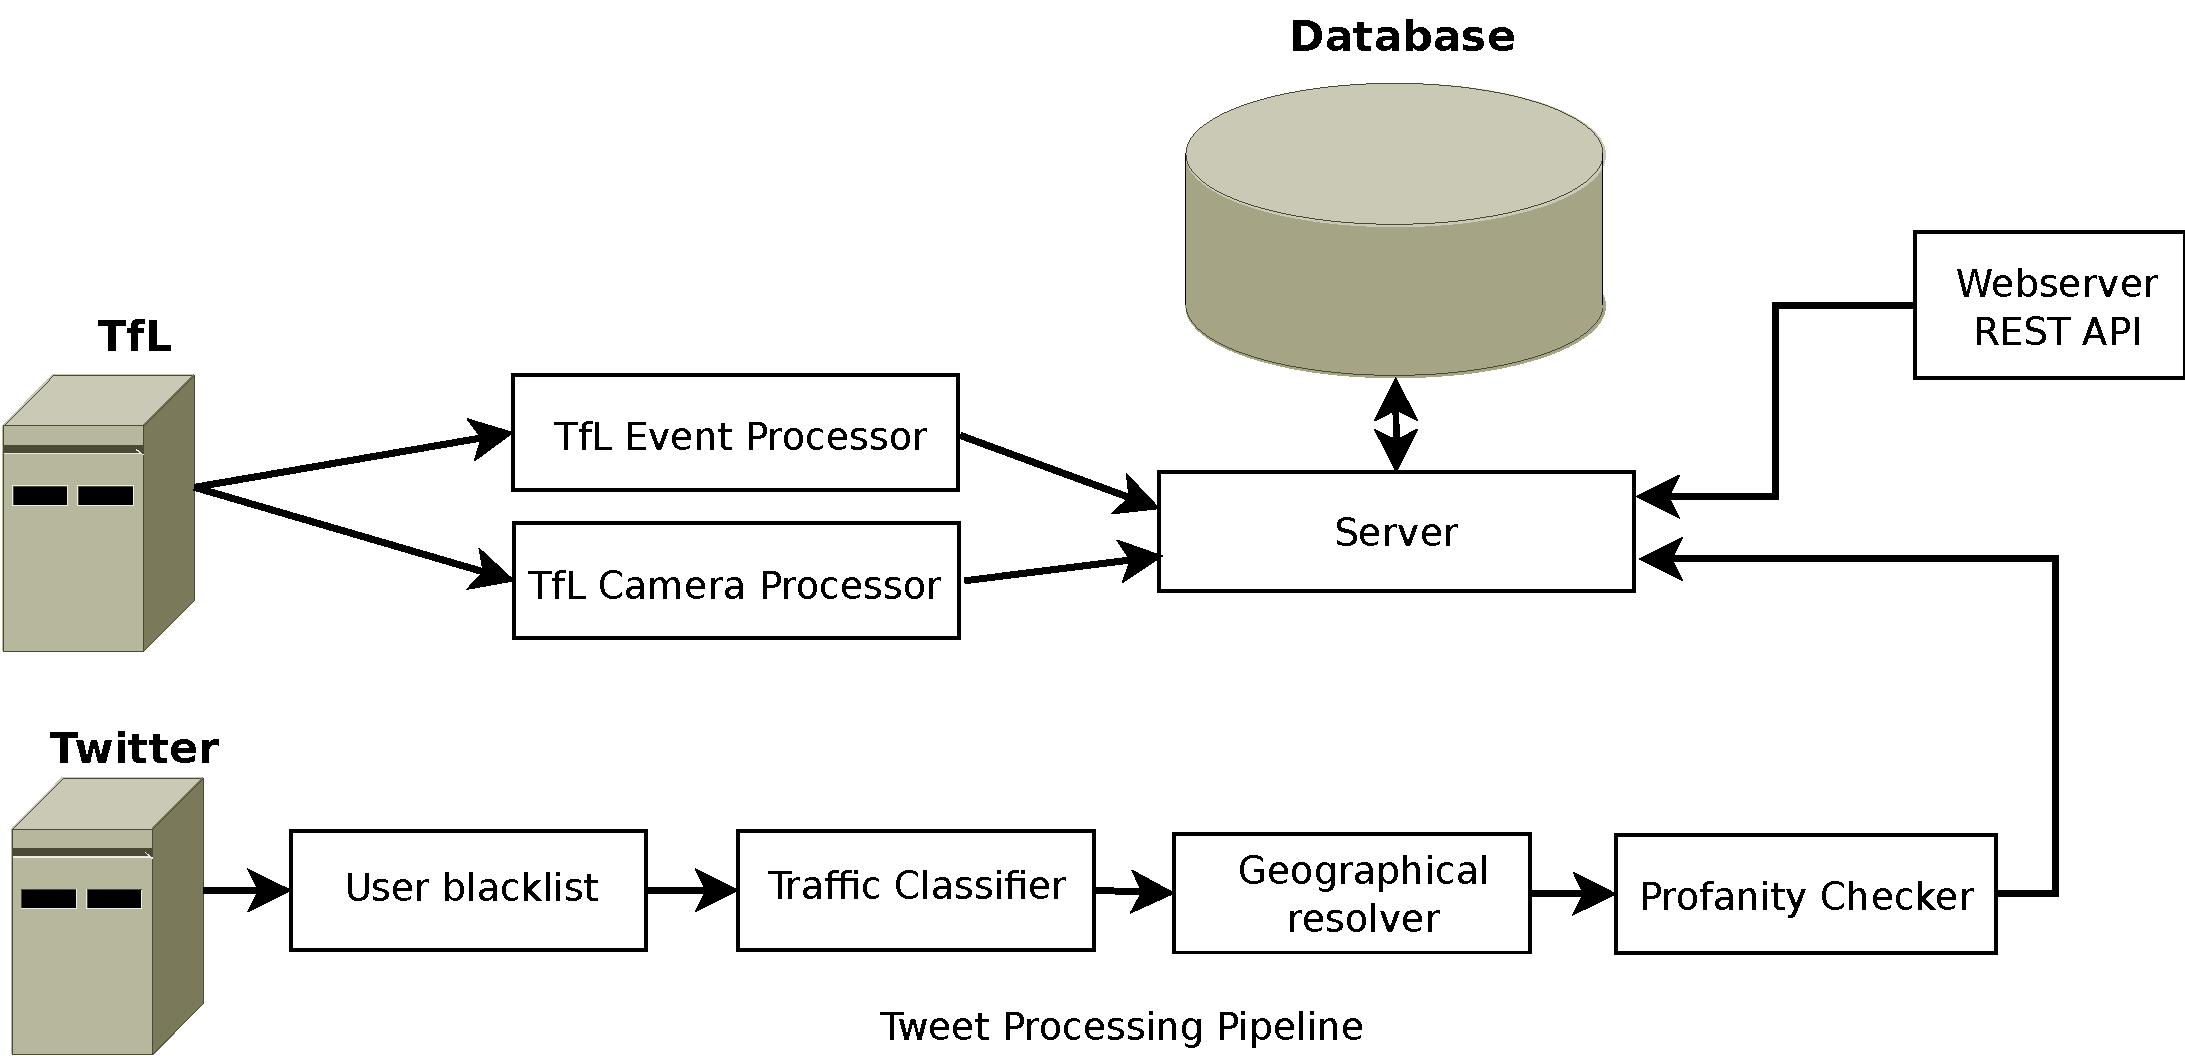
\includegraphics[width=1\textwidth]{images/design/server/server.pdf}
\caption{Server Design}
\label{fig:server_design}
\end{figure}

\subsubsection{Data acquisition}
The sources that we collect data from are Transport for London (TfL) and Twitter.

\paragraph{1. TfL Disruption Events}
The TfL website provides different types of data feeds that can be used to obtain information relevant to traffic. 
One of the TfL data feeds we use is the "live traffic disruptions". This provides information about traffic disruption events in the area of London. This information contains details about the severity of the event, the type (e.g. road works, signal failure, accident), the location and an estimated time for the event's end.

\paragraph{2. TfL Traffic Cameras}
To provide a more complete view around the area of the event we also store the "live traffic camera images" feed from TfL. This provides URLs to pictures taken by traffic cameras within the last 15 minutes as well as the location of the camera and the timestamp when the picture was taken.

\paragraph{3. Twitter}
For Twitter we defined the area around London that we are interested to collect tweets from. In addition to this, we used a search query with the words that we want the results from Twitter to contain. This query is consisted of words chosen after experimentation.

\subsubsection{Data analysis}
\paragraph{1. TfL Feeds Processing}
The TfL feeds we used for the application are returned as XML files. Using the minidom python library, we were able to parse them. Because a TfL traffic event's position is returned as a point in British national grid coordinates, we first transform them to longitude and latitude coordinates before storing them in the database. This is done using a python module that implements the algorithm given in the ordnance survey guide.\cite{website:grid2lonlat_alg} \cite{website:grid2lonlat_impl}

\paragraph{2. Twitter Processing}
In contrast to the TfL, the Twitter data are returned in a JSON format. For this reason, we used the python-twitter API which saves the JSON information into classes and variables that can then be easily accessed. Before storing the tweets to the database each of them passes through a processing pipeline.

First, the username of the person who sent the tweet is checked to find out if he is in the blacklist. The blacklist is a txt file we have in the server which can contain different usernames for twitter accounts from which we do not want to store tweets. The reason for this is that we can use this blacklist for traffic (or other) bots so that we only have real persons' tweets in the database. Then, we use the classifier to decide if the tweet's text is about traffic or not. The process of classification is described in the Classification section. After classifing a tweet as traffic, we use a regex to find any streets or roads in its text. Finally, before storing the tweet we check a list of words that we have in a txt file to determine if they are included in the message. This is implemented for a profanity filter.

\textbf{Soundex}

Terms that are often misspelled can be a problem for the tweet parsing. For example, the street name `Cannon street' can have strange spelling such as `Canoon street'. To avoid this problem, this project introduces Soundex algorithm which is a phonetic algorithm for indexing names by sound, as pronounced in English. Its goal is for homophones to be encoded to the same representation so that they can be matched despite minor differences in spelling. The algorithm mainly encodes consonants; a vowel will not be encoded unless it is the first letter. That means a misspelled street name probably matches the right street name if the first letter in the street name is not typed wrongly.\\
In the project, a table which stores street addresses is created for looking up geolocation. If a tweet doesn't have property called `geolocation', it will be parsed to extract its street address. However, some extracted addresses have no corresponding geolocation in the database because there are misspells in them. The misspell street address is split into independent words in which the white spaces are removed. Then those words are encoded using Soundex algorithm to get Soundex codes which are combined into a string. This string is called Soundex string. This Soundex string is matched with other Soundex strings of the street addresses which are stored in the database. This algorithm improves the ratio of street address matching.


\subsubsection{Storage}
For the storage of data we use a PostgreSQL database. This decision was made because PostgreSQL is one of the most stable open source database management systems. Due to the large amount of database queries, we needed to use an efficient way to store and analyze the information we acquired from the TfL feeds and Twitter. For this reason, we decided to use a Geographic Information System called PostGIS, which is a spatial database extension for PostgreSQL. This allowed us to store geolocations (longitude and latitude) as points.

With the use of PostGIS, queries to the database became easier and more efficient. The use of functions provided by PostGIS, such as \emph{ST\_DWithin} to find all points around a route or a point within a radius, or \emph{ST\_Distance} to find the distance between two points, made all queries simpler. In addition, the main advantage of PostGIS is that it uses generalized search trees (GiST) to index the geometries. 

A GiST like a B-tree uses key-pointer pairs. The difference with B-trees is that a GiST key is a user-defined data type. This allows different types of operations, rather than simple comparisons, such as nearest-neighbor searches and statistical approximations over large data sets. In PostGIS, the GiST is used for spatial indexing by allowing the index to use a bounding box for each geometry (e.g. line) instead of storing the whole geometry in it. Therefore, with bounding box comparison, instead of comparing geometries, functions such as ST\_DWithin are made more efficient. \cite{website:postgis_stdwithin}

For the project we used the following tables:
\begin{itemize}
\item Tables used by the final application
  \begin{itemize}
  \item \emph{tfl}: The current tfl disruption events
  \item \emph{archive}: To store old tfl disruption events for further analysis
  \item \emph{tflcameras}: The current camera pictures' url
  \item \emph{tweets}: To store the traffic tweets acquired from twitter
  \item \emph{geolookup}: Used to store addresses with their Soundex value and their geolocation which is acquired from Google Maps
  \item \emph{tweets\_metrics}: Used to store different types of metrics for the tweets
  \end{itemize}
\item Tables used to train the classifier
  \begin{itemize}
  \item \emph{labelled\_tweets}: To store manually labelled tweets as traffic or non-traffic
  \item \emph{stop\_words}: Words that can be removed before data analysis
  \end{itemize}
\item Tables used by PostGIS
  \begin{itemize}
  \item \emph{geography\_columns}: This is a view that shows all the columns of the database that use geography points
  \item \emph{spatial\_ref\_sys}: A list of spatial reference systems and details to transform between them
  \end{itemize}
\end{itemize}

\subsubsection{Interface}

Before the server implementation, the creation of a mock server api was essential. This 
provided us with the ability to seperate the work on the application and server design from the very 
beginning of the project. At this stage, the rest endpoints had to be defined in order to agree on the 
data format that was transferred between the server and the client. The next thing was creating mocked 
JSON data for responding to the requests. Such data included fixed sets of disruptions, tweets and 
cameras.

The server consists of several threads. Three of these threads are used to collect the data feeds from TfL and messages from Twitter, as described in a previous section. Another thread is used by the Representational State Transfer (REST) server to receive and respond to mobile client requests. The reason for the implementation of the different threads is to achieve a fault resilient server. If one of these threads stops working because of an unexpected error, the remaining threads can continue to work unaffected. Furthermore, each thread stores a log to a file about its actions and errors it has encountered, which makes debugging simpler.

The REST server can receive GET or POST requests from the mobile client. If the request was not in the correct format then the server returns a bad request (Error 400). The response to these requests is a JSON file. 

The server and the mock server can run at the same time on different ports. Each request uses a URL that has the version written in it. This achieves old version compatibility, as the server can continue to support previous client versions. In the following requests the version is named 0.2:
\begin{itemize}
\item \emph{GET} \url{/t4t/0.2/disruptions} \\
Parameters: \emph{longitute, latitude, radius, closestcam (optional)} \\
Description: A request that returns all current disruptions in an area defined by a point (longitude and latitude) and a radius. There is also an option to return only the closest camera for each request.

\item \emph{GET} \url{/t4t/0.2/disruptions} \\
Parameters: \emph{topleftlat, topleftlong, bottomrightlat, bottomrightlong, closestcam (optional)} \\
Description: A request that returns all current disruptions in an area defined by 2 points that are the 2 opposite corners of a rectangle. There is also an option to return only the closest camera for each request.

\item \emph{GET} \url{/t4t/0.2/disruptions/route} \\
Parameters: \emph{JSON encoded list points on a route} \\
Description: A request that posts a json file of points on a route that will return all disruptions around it.

\item \emph{GET} \url{/t4t/0.2/tweets} \\
Parameters: \emph{disruptionID, filter (optional)} \\
Description: A request that returns all tweets that are around a disruption event. There is also an option to use the profanity filter for the tweets that are returned.

\item \emph{GET} \url{/t4t/0.2/tweets} \\
Parameters: \emph{longitute, latitude, radius, filter (optional)} \\
Description: A request that returns all tweets in a area defined by a point (longitude and latitude) and a radius. There is also an option to use the profanity filter for the tweets that are returned.

\item \emph{GET} \url{/t4t/0.2/cameras} \\
Parameters: \emph{disruptionID, closestcam (optional)} \\
Description: A request that returns all cameras that are around a disruption event. These requests have an option to return only the closest camera.
\item \emph{GET} \url{/t4t/0.2/cameras} \\
Parameters: \emph{longitute, latitude, radius, closestcam (optional)} \\
Description: A request that returns all cameras in a area defined by a point (longitude and latitude) and a radius. These requests have an option to return only the closest camera.

\end{itemize}
